\documentclass{beamer}
\usepackage{graphicx}
\usepackage{amsmath}
\usepackage[utf8]{inputenc}

\usetheme{Warsaw}
%\title[Make a LaTeX presentation using Beamer]{Introduction  to Beamer\\How to make a presentation with LaTeX?}
\title{Pythagorean Hodograph curves}
\author{Aki Reijonen}
%%\institute{Math-linux.com}
%%\date{July 13, 2007}
\begin{document}

\begin{frame}
\titlepage
\end{frame}


% arc length
%
% rational offsets
% C^1 hermite interpolation
\begin{frame}{Introduction}

Arc length of polynomial plane curve $r : [0,1] \to \mathbb{R}^2, r(t) = (x(t), y(t)$:
\[
  length(r) = 
\int_0^1 ||r'(t)||^2 dt = \int_a^b \sqrt{x'^2(t) + y'^2(t)} dt
\]

In general the integral doesn't have a closed form solution.

\end{frame}

\begin{frame}

\begin{definition}[Pythagorean hodograph property]
Polynomial plane curve $r(t)=(x(t), y(t))$ has a pythagorean hodograph if 
there exists a non-negative polynomial $\sigma(t)$ such that

\[
  ||r'(t)||^2 = x'(t)^2 + y'(t)^2 = \sigma^2(t)
\]
\end{definition}
\pause

PH curves are exactly the curves for which the arc length function is a polynomial:
\[
  length(r) = \int_0^1 \sqrt{x'^2(t) + y'^2(t)} dt = \int_0^1 \sigma(t) dt
\]

\end{frame}

\begin{frame}
\frametitle{Cubic PH curves}

\begin{figure}
\centering
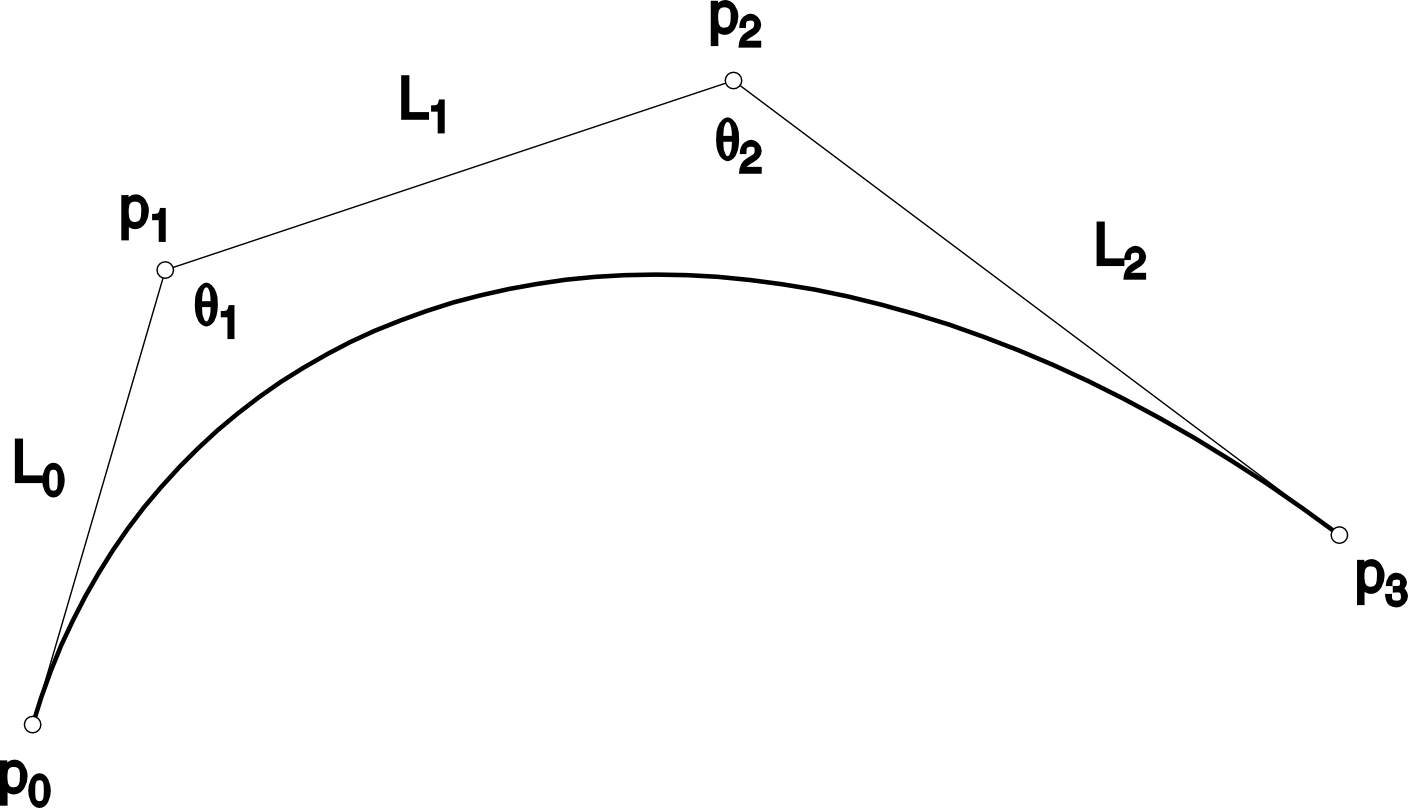
\includegraphics[width=\textwidth]{cubic_ph_bezier.png}
\end{figure}

In Bézier form, cubic PH curves need to satisfy the conditions:
\begin{itemize}
\item $L_1 = \sqrt{L_2 L_0}$
\pause
\item $\theta_0 = \theta_1$
\end{itemize}
\end{frame}


\begin{frame}

Some properties of PH curves:
\begin{itemize}
  \item Unit tangent is rational: $r'(t)/||r'(t)|| = (x'(t), y'(t))/\sigma(t)$
  \pause
  \item Unit normal is rational: $(2x'(t)y'(t), y'^2(t) - x'^2(t))/\sigma(t)$
  \pause
  \item Curvature is rational: $2(x'(t)y''(t) - x''(t)y'(t))/\sigma(t)$
  \pause
  \item Offset curves $r_d(t) = r(t) + dn(t)$ are rational curves (of degree $2n-1$)
  \pause
  \item Degree is always odd
  \pause
  \item Everything is easier 
\end{itemize}

\end{frame}

\begin{frame}
\frametitle{Hermite interpolation}

\begin{itemize}

\item Quintic PH curves can solve the first-order Hermite interpolation problem:
Given values for $r(0),r(1)$ and $r'(0), r'(1)$, find a PH curve that agrees.
\pause
\item Ordinary cubics have a unique solution.
\pause
\item For quintic PH curves, there are four solutions:
\end{itemize}
\begin{figure}
\centering
\vspace{-8mm}
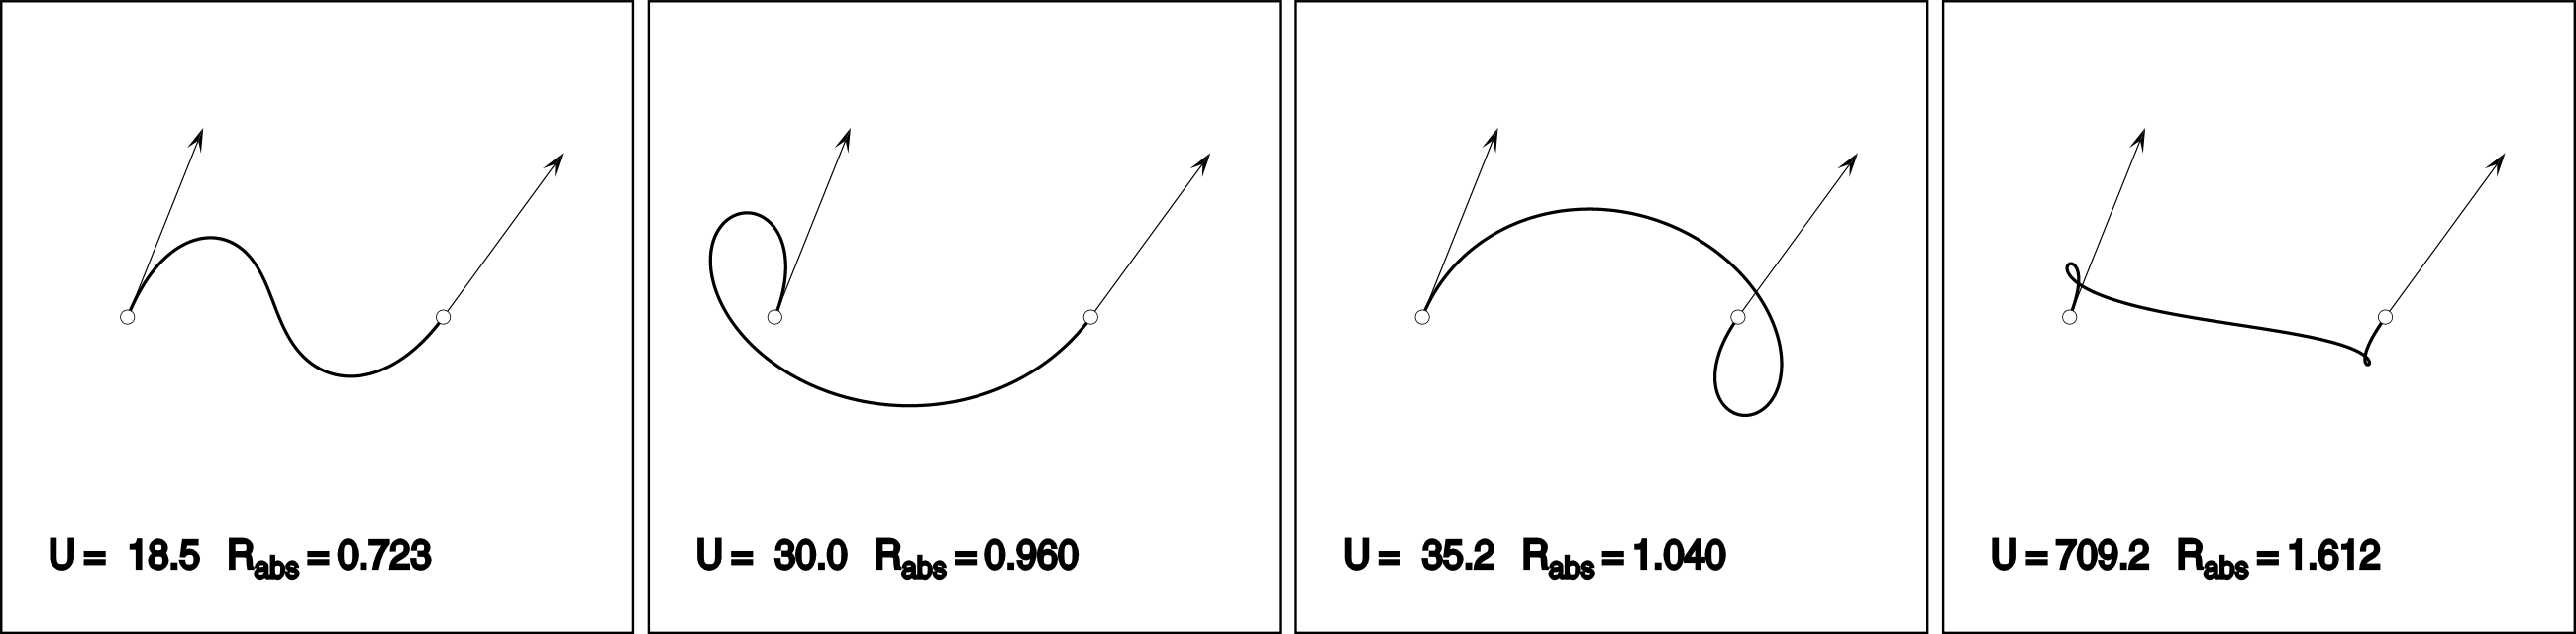
\includegraphics{ph_curve_hermite_solutions.png}
\end{figure}
\vspace{-2mm}
\pause
Alternative ways:
\begin{itemize}
  \item A pair of cubic PH curves
  \pause
  \item A cubic PH composed with a möbius transformation
\end{itemize}
\end{frame}

\begin{frame}

\begin{figure}
\centering

\frametitle{Comparison with cubic interpolants}

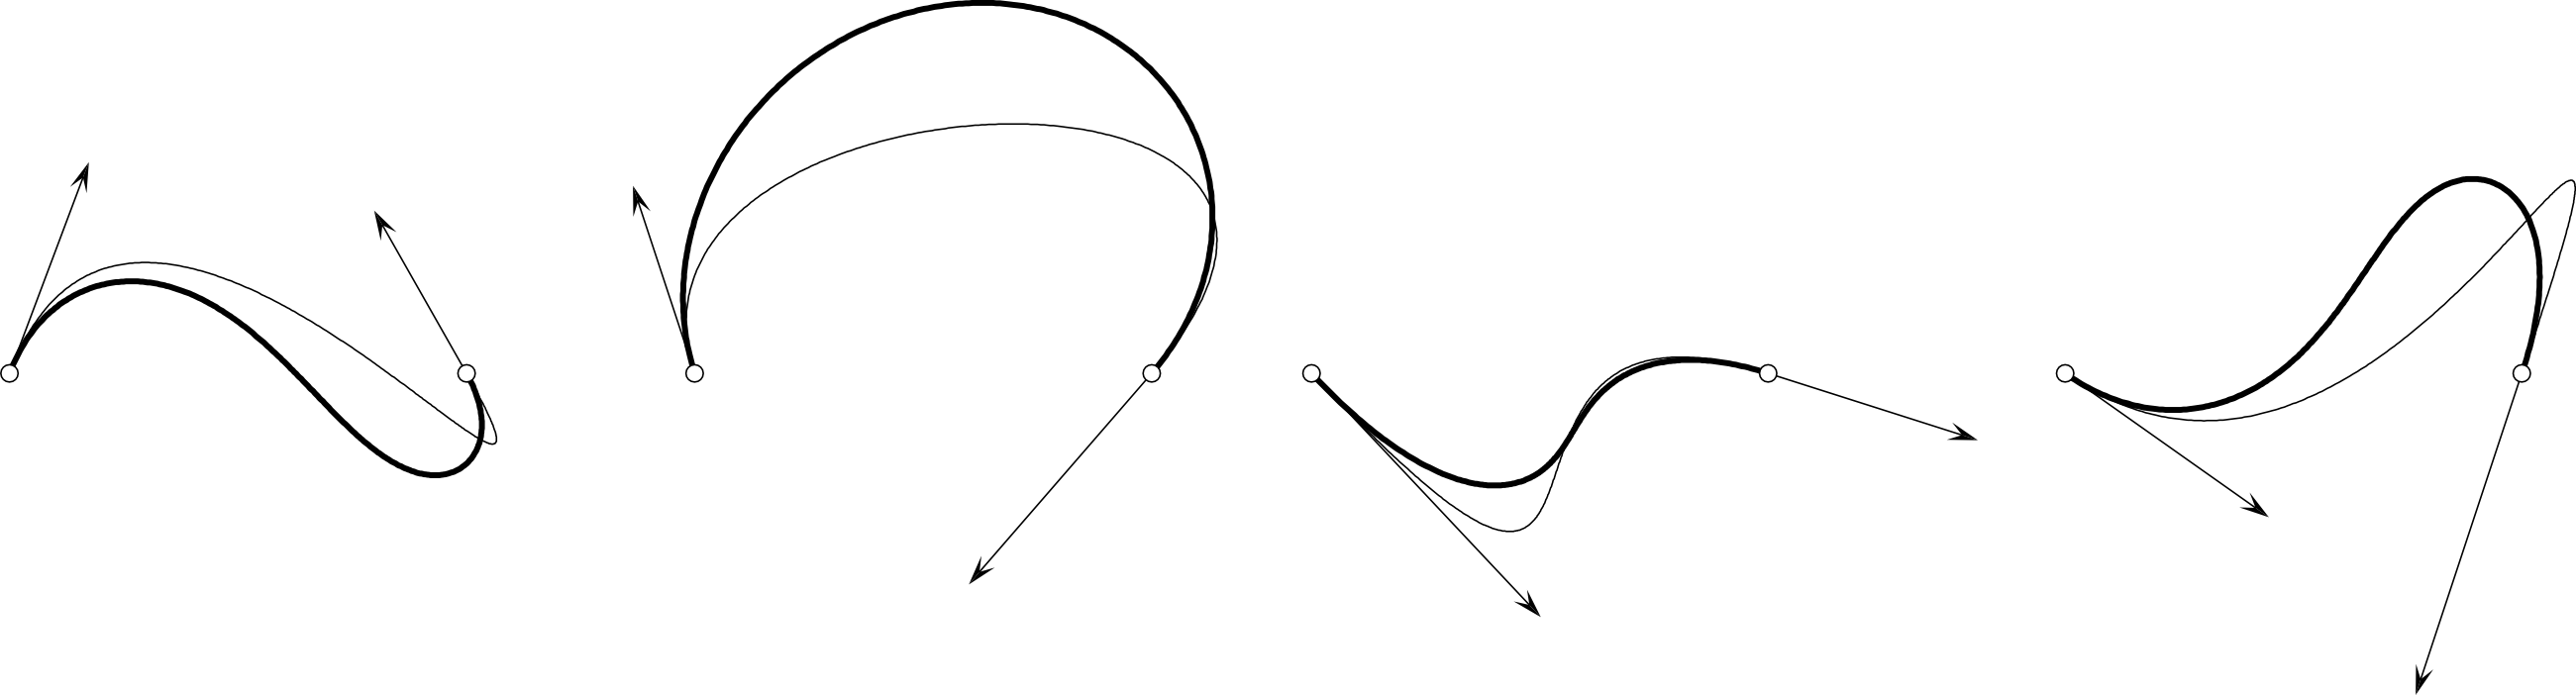
\includegraphics{hermite_vs_cubic.png}
\end{figure}

\end{frame}

\begin{frame}

\frametitle{Minkowski PH curves}

Defined in Minkowski space $\mathbb{R}^{2,1}$ which has indefinite inner product:
\[
\langle (u_0, u_1, u_2), (v_0, v_1, v_2) \rangle = u_0v_0 + u_1v_1 - u_2v_2
\]

\pause
PH property for the curve $m(t) = (x(t), y(t), r(t)) : [0,1] \to \mathbb{R}^{2,1}$:
\[
\langle m', m' \rangle = x'^2(t) + y'^2(t) - r'^2(t) = \sigma^2(t)
\]

\pause
Motivation: interpret $(x(t), y(t), r(t)$ as a circle of radius $r(t)$ at $(x(t), y(t))$
\end{frame}

\begin{frame}
Minkowski distance defined by: $d(u,v)^2 = \langle u-v, u-v \rangle$

\begin{figure}
\centering
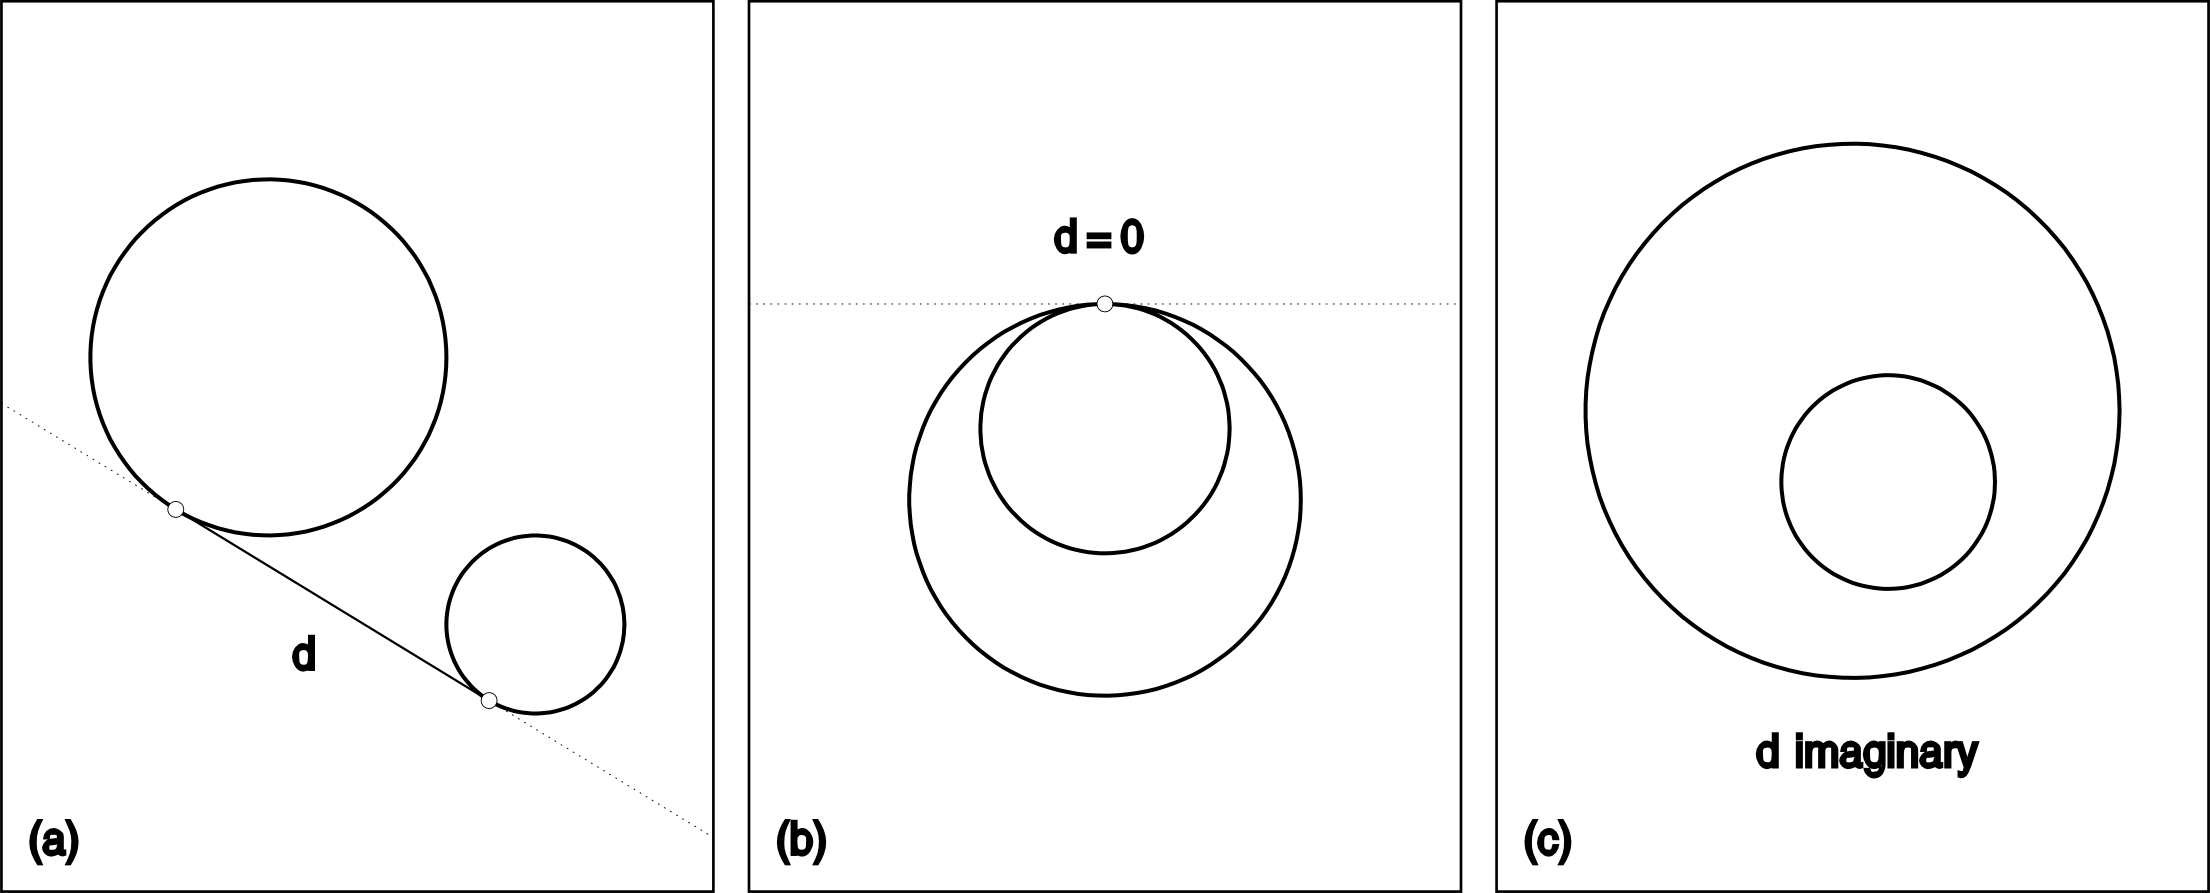
\includegraphics[width=\textwidth]{minkowski_metric.png}
\end{figure}
\end{frame}

\begin{frame}
\frametitle{Medial Axis Transform}

\begin{figure}
\centering
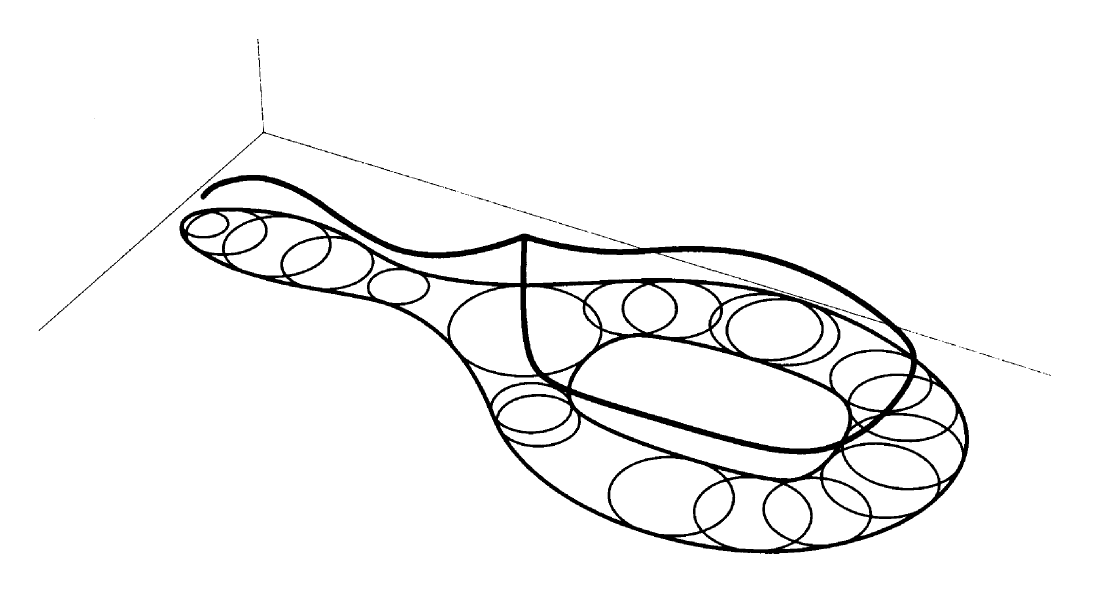
\includegraphics[width=\textwidth]{mat_mph.png}
\end{figure}

MAT as a graph of MPH curves
\end{frame}

\begin{frame}
\frametitle{MAT offset curve trimming}

\begin{figure}
\centering
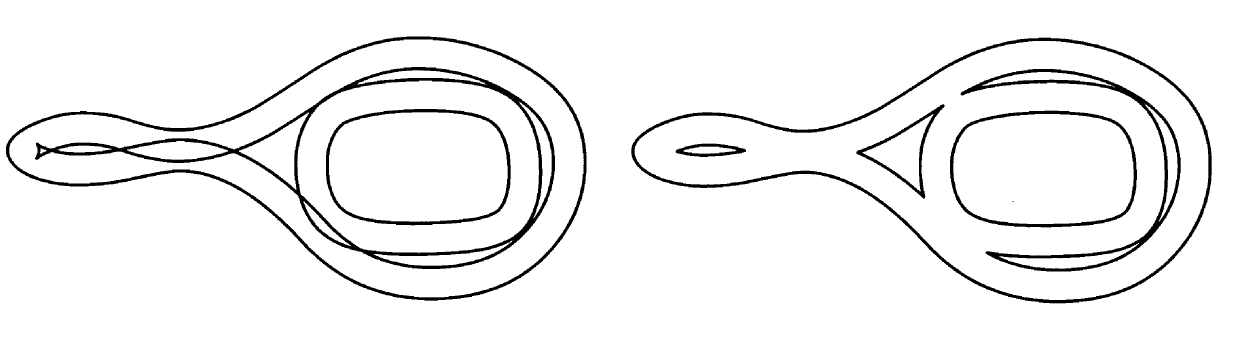
\includegraphics[width=\textwidth]{untrimmed_trimmed.png}

Untrimmed / trimmed offset curves
\end{figure}

\end{frame}

\end{document}
